\documentclass{article}
\usepackage[utf8]{inputenc}
\usepackage{graphicx}
\usepackage{float}

\title{Multi Agent System approach. A road to robot cooperation}
\author{}
\date{February 2020}

\begin{document}

\maketitle

\section{Introduction}
\section{Multi Agent Systems:an overview}
\section{Reinforcement Learning aproach for 
coordination}
\subsection{Theoretical formulation}
Inside the machine learning methods we can find 3 different big types:
\begin{itemize}
\item Supervised Learning. Inferring a regression or classification through a labeled trainging data
\item Unsupervised Learning. Inferring from datasets without labels.
\item Reinforcement Learning. Study how an agent must behave in order to maximize the cumulative reward. 
\end{itemize}  
Thiss last type is what we will exploitf. It is the best scenario when we have an idea of which actions are "good" and "bad" and we want to maximize the goodness of our agent. Let's go through the theory and algorithms used in this paradigm.
\newline
In our framework we will have an agent that does the decision making and everything out of the agent is the environmnent. The environment is responsible to offer a response for each action the agent takes, providing a new environment state and the reward for the action the agent took (See figure 1). They interact continuouslly.
\newline
Lets state this in a more formal way.
We have a set of states $\mathcal{S}$. Initially our agent starts at a determined state $ s \subseteq \mathcal{S}$. For the sake of simplicity lets denote $S_{t}$ the state the Agent is at the $t$ timestep. For each state $S_{t}$ we have a set of actions the agent can take $A(S_{t})$. Once the agent has chosen an action the environment returns a new state $S_{t+1}$ and a reward $R_{t+1}$. \newline
\newline
\begin{figure}[H]
\centering 
$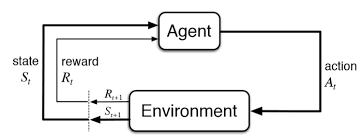
\includegraphics[scale=0.7]{agent_environment.png}$
\caption{Agent-Environment diagram}
\end{figure}
The agent learns a policy $\pi(a|s)$ that at every state assigns a probability of each action available in this state of being chosen. This policy keeps changing over experience and our goal is to build a policy that maximizes the cumulated reward from the initial to the terminal state. 
\newline
How can we maximize the total reward? 
\newline Lets denote $G_{t} = R_{t+1} + R_{t+2} + R_{t+3} + \dots $ If our interactions go over infinity we will use the discounted return in order to make them finite.\newline
$G_{t} = R_{t+1} + \gamma R_{t+2} + \gamma^{2} R_{t+3} + \dots + R_{T} = \sum_{i = 0}^{\infty}\gamma^{i} R_{t+1+i} $ choosing a $\gamma < 1$. If the rewards are bounded we can easily see this series is convergent. We chose $\gamma < \delta < 1$ and we see that $$\lim_{i\to\infty}\frac{\delta^{i}}{\gamma^{i}*R_{t+1+i}} = \lim_{i\to\infty}(\frac{\delta}{\gamma})^{i} * \frac{1}{R_{t+1+i}} = \infty$$ since it is the exponential of a number bigger than 1 multiplied by a bounded series. That means that from a point of the series the second series is bigger than the first, since the second series is the geometric series of $\delta$ and we know it is convergent, so it is the first one.
\newline
The parameter $\gamma$ can also be used in non infinite tasks. In a sense it is a way of weighting the rewards. If $\gamma$ is close to $ 1$ we want each reward to count the same. If $\gamma$ is close to $0$ we want the first rewards to count more than the next ones in the task.

\end{document}
